\documentclass{article}
\usepackage[paperheight=14.5mm,paperwidth=257mm,margin=0in]{geometry}
\usepackage[ngerman]{babel}

\usepackage{rotating}

\usepackage{charter}
\usepackage[charter]{mathdesign}
\usepackage[scaled=.95]{helvet}
\renewcommand{\familydefault}{\sfdefault} % sans serif, as modern titles are set
\usepackage[T1]{fontenc} % T1 Schrift Encoding
\usepackage{textcomp}	 % Zusatzliche Symbole (Text Companion font extension)

% To show the boxes used in this document define a non-white color here
\usepackage{xcolor}
\newcommand{\boxcol}{white}

\begin{document} %
% Name and title are rotated by 180 degrees: the spine reads from bottom to top when the book stands upright.
% Logo and year stay at the bottom, so the name (the start of the text) ends up next to them.
\vspace{-5pt} %
\noindent\raisebox{-2pt}{\rotatebox[origin=c]{180}{%
% Name
\fcolorbox{\boxcol}{white}{%
\begin{minipage}{\dimexpr0.15\textwidth-2\fboxrule-2\fboxsep\relax}
\begin{center}
{\Large Author Name}
\end{center}
\end{minipage}}%
%
% Title
\fcolorbox{\boxcol}{white}{%
\begin{minipage}{\dimexpr0.75\textwidth-2\fboxrule-2\fboxsep\relax}
\begin{center}
\vspace{3pt} % No idea why this is not aligned correctly
{\Large Titel der Dissertation}
\end{center}
\end{minipage}}}}%
%
% Logo
\noindent\fcolorbox{\boxcol}{white}{%
\begin{minipage}{\dimexpr0.06\textwidth-2\fboxrule-2\fboxsep\relax}
\begin{center}
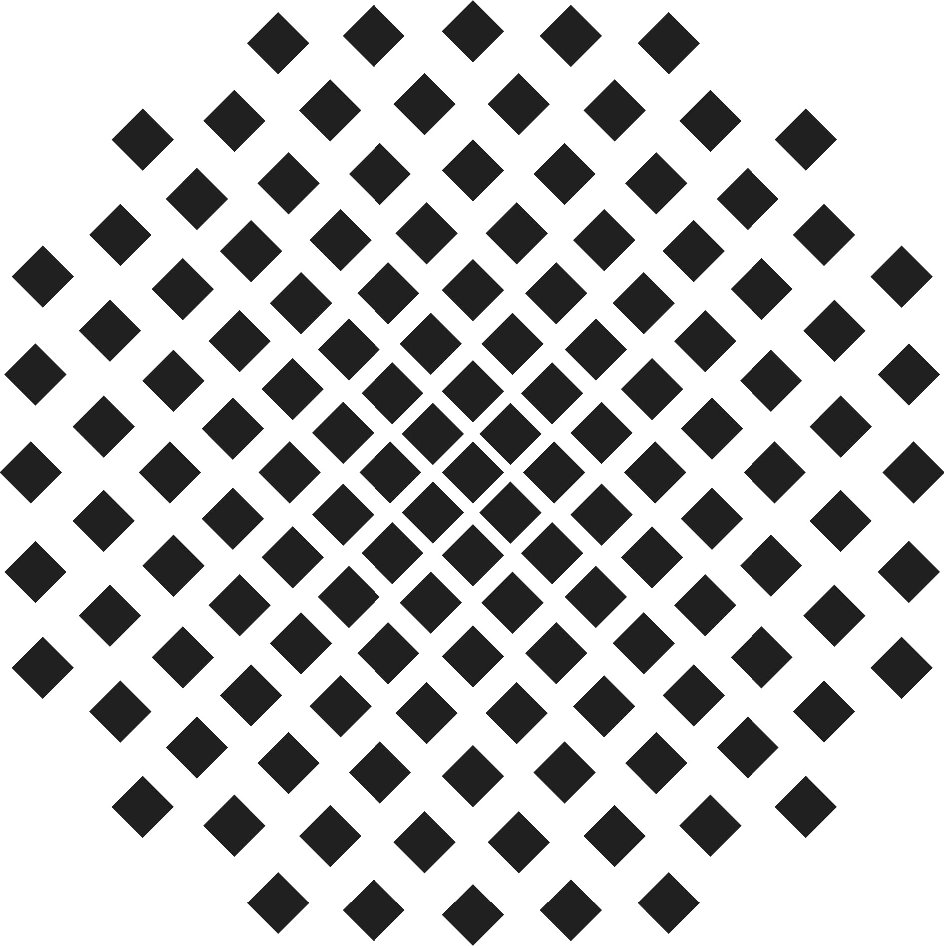
\includegraphics[height=1cm]{../shared/ustutt-logo-only}
\end{center}
\end{minipage}} %
%
% Year
\noindent\fcolorbox{\boxcol}{white}{%
\begin{minipage}{\dimexpr0.04\textwidth-2\fboxrule-2\fboxsep\relax}
\rotatebox{90}{{\large 2015}}
\end{minipage}}

\end{document}
